\chapter{Theory}
\label{c:theory}

\section{Standard Model}

The standard model (SM) is a theory which describes the fundamental particles and their interactions. Matter consists of six quarks and six leptons, each of which has an anti-particle with opposite sign quantum numbers. They are organised into three generations each of which contains heavier particles than the last, as seen in Table~\ref{table:SMmatter}. All of the stable matter in the universe is made up of particles from the first generation, ie. quarks make up protons and combined with electrons they form atoms. The leptonic sector consists of charged leptons, which can interact via the electromagnetic and weak forces, and neutrinos, which interact via the weak force only. The neutrinos are assumed to be massless in the standard model however observations of neutrino oscillations revealed that neutrinos have mass.

\begin{table}[ht!]
\centering
\caption{Quarks and leptons}
\label{table:SMmatter}
\footnotesize
\begin{tabular}{|c|l|l|l|l|l|l|}
\hline
\multirow{2}{*}{Generation} & \multicolumn{3}{c|}{Quarks}                             & \multicolumn{3}{c|}{Leptons}              \\ \cline{2-7} 
                            & Flavour & Charge & Mass (MeV)                           & Flavour      & Charge & Mass (MeV)        \\ \hline
\hline

\multirow{2}{*}{I}          & u       & 2/3    & $2.2^{+0.6}_{-0.4}$                  & e            & -1     & 0.511             \\
                            & d       & -1/3   & $4.7^{+0.5}_{-0.4}$                  & $\nu_{e}$    & 0      & $<2\times10^{-6}$ \\ \hline
\multirow{2}{*}{II}         & c       & 2/3    & $(1.27\pm 0.03)\times10^{3}$         & $\mu$        & -1     & 105.66            \\
                            & s       & -1/3   & $96^{+8}_{-4}$                       & $\nu_{\mu}$  & 0      & $<0.19$           \\ \hline
\multirow{2}{*}{III}        & t       & 2/3    & $(173.21\pm0.51\pm0.71)\times10^{3}$ & $\tau$       & -1     & $1776.86\pm0.12$  \\
                            & b       & -1/3   & $(4.18^{+0.04}_{-0.3})\times10^{3}$  & $\nu_{\tau}$ & 0      & $<18.2$           \\ \hline
\end{tabular}
\end{table}

Quarks interact via the electromagnetic or strong force. Each quarks has an electric charge, as seen in Table~\ref{table:SMmatter}, and carries a colour charge of red, green or blue, where all three colours combined form a colour-singlet state. A combination of quarks with a colour and it's anti-colour can also form a colour-singlet state. The theory of colour confinement means that quarks can only be found in colour-singlet states such as in bound states of baryons or mesons. 
The top quarks is the heaviest quark with a mass approximately equivalent to a lead nuclei. The top quark is the only quark which predominantly decays before it hadronises due to it's short lifetime of $5\times10^{-25}$~seconds. The main decay mode for top quarks is to a bottom quark and a W boson which occurs $95.6\pm3.4\%$ of the time.
Finally, the force carriers consist of gauge bosons of integer spin, as seen in table~\ref{table:SMbosons}. Photons and Z bosons can mediate neutral electroweak interactions whereas W bosons can mediate charged electroweak interactions. The gluons mediate the strong interaction and occur with 8 different types of colour charge which will be described in section~\ref{subsec:QCD}. 
The Graviton is hypothesised to carry the gravitational force but there is as yet no evidence to support this hypothesis.
\begin{table}[ht!]
\centering
\caption{Gauge bosons}
\footnotesize
\label{table:SMbosons}
\begin{tabular}{|l|l|l|l|l|l|}
\hline
Gauge boson                       & Force           & Charge & Mass (GeV) & Spin & Range (m)  \\ \hline \hline
Photon ($\gamma$)                 & electromagnetic & 0      & 0          & 1    & $\infty$   \\ \hline
W$^{\pm}$                         & weak            & $\pm1$ & $80.385\pm0.015$           & 1    & $10^{-18}$ \\ \hline
Z                                 & weak            & 0      & $91.1876\pm0.0021$           & 1    & $10^{-18}$ \\ \hline
gluon                             & strong          & 0      & 0          & 1    & $10^{-15}$ \\ \hline
Graviton\footnote{hypothesised} & gravitational   & 0      & 0          & 2    & $\infty$   \\ \hline
\end{tabular}
\end{table}

The discovery of the Higgs boson in 2012 completed the standard model with an explanation of how the fundamental particles have mass via the electroweak symmetry breaking mechanism.

\subsection{Electroweak theory}

\subsubsection{QED}
\label{subsec:QED}

Figure~\ref{fig:QEDvertex} shows the fundamental QED vertex where a charged particle (charged lepton or quark) and charged anti-particle interact with a photon. The convention in this thesis is that time flows from left to right. However, these diagrams may be rotated as long as they conserve energy. Hence, this diagram includes electron-positron annihilation into a photon, a photon pair-producing an electron-positron pair, an electron emitting a photon or a positron emitting a photon depending on the orientation of the diagram (if we assume that the charged particles are first generation charged leptons). 

\begin{figure}[ht!]
\begin{center}
    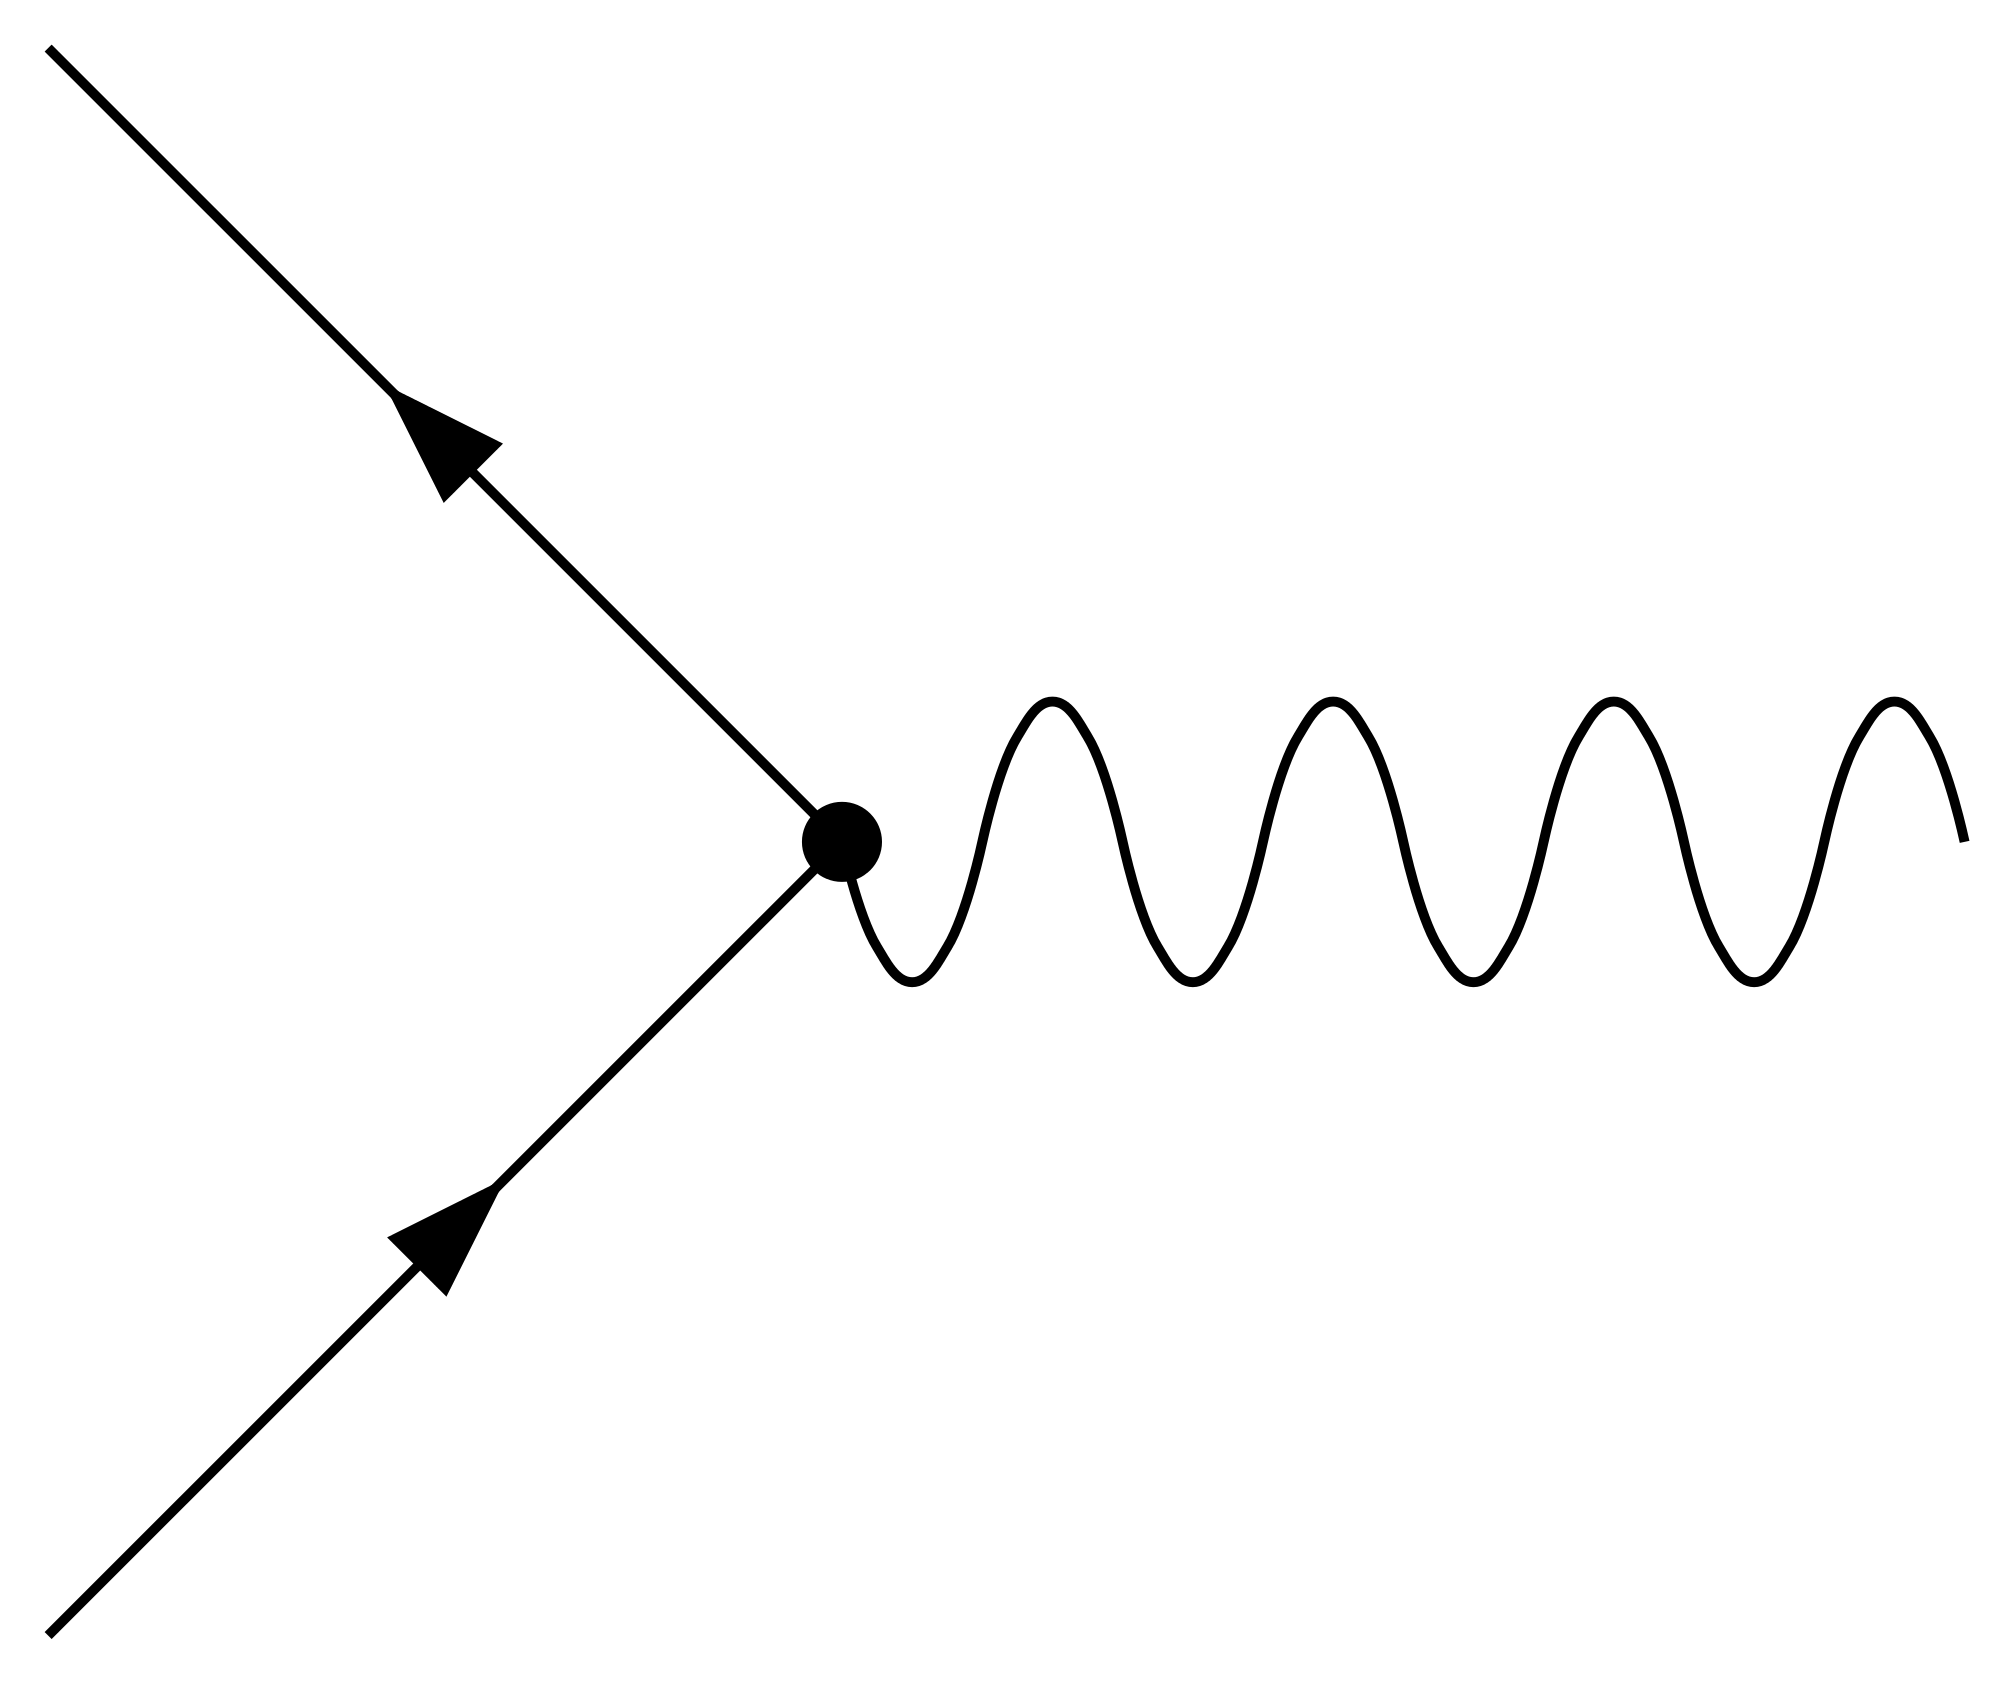
\includegraphics[width=0.35\textwidth]{images/Theory/QEDvertex.png}
    \caption{Fundamental QED vertex}
    \label{fig:QEDvertex}
\end{center}
\end{figure}

This diagram alone cannot occur as it violates conservation of energy but it can be used to build a full Feynman diagram for a particle physics process. QED interactions conserve lepton or quark flavour. 
The QED Lagrangian can be found in Eq.~\ref{eqn:QEDL} with $D_{\mu}$ representing the covariant derivative which is defined as $D_{\mu} = \partial_{\mu} + iqA^{\mu}$, where $A^{\mu}$ is the four-potential of the electron and $q$ is the charge. The mass of the particle is represented by $m$ and $F_{\mu\nu}$ is the electromagnetic field tensor.

\begin{equation}
\mathcal{L} = \overline{\phi}\left(i\gamma^{\mu}D_{\mu}-m\right)\phi - \frac{1}{4}F_{\mu\nu}F^{\mu\nu}
\label{eqn:QEDL}
\end{equation}
This Lagrangian is gauge invariant, ie. it is invariant under U(1) phase transformations, where U(1) is the unitary group of complex numbers. Application of the Euler-Lagrange equations leads to the derivation of the Dirac Equation shown in Eq.~\ref{Eqn:Dirac}.

\begin{equation}
i\hbar \gamma ^{\mu }\partial _{\mu }\psi -mc\psi =0
\label{Eqn:Dirac}
\end{equation}

\subsubsection{Weak interactions}

The charged weak interaction is the only interaction where a flavour changing process can occur. The diagram of weak nuclear decay in Fig.~\ref{fig:QEDvertex} illustrates the W boson's interaction with different flavour quarks and leptons.


\begin{figure}[ht!]
\begin{center}
    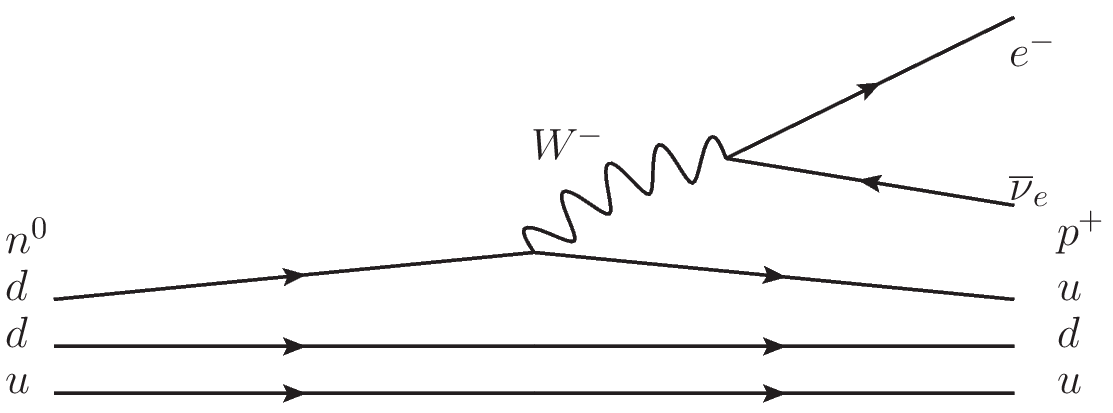
\includegraphics[width=0.65\textwidth]{images/Theory/weakDecay.png}
    \caption{Weak nuclear decay of neutron to proton}
    \label{fig:QEDvertex}
\end{center}
\end{figure}

Z bosons partake in neutral weak interaction where they can interact with any quark or lepton as long as the flavour is conserved at the vertex.

\subsubsection{Electroweak Unification}

Glashow, Weinberg and Salam formulated the unification of the weak and electromagnetic forces combined in the SU(2)~x~U(1) gauge group. They are hypothesised to merge into one electroweak force above the unification energy of $\approx 100$~GeV. The theory contains four gauge bosons, three W bosons W$_{a}~(a=1,~2,~3)$ and one B boson. The spontaneous symmetry breaking mechanism proposed by Higgs, Brout and Englert results in the linear combination of these 4 bosons into the four more familiar gauge bosons, W$^{\pm}$, Z and the photon ($\gamma$) as shown in Eqs.~\ref{eqn:Zgamma} \&~\ref{eqn:Wpm}, where $\theta_{W}$ is the weak mixing angle.

\begin{equation}
\label{eqn:Zgamma}
\left( \begin{array}{c}
\gamma \\
Z \end{array} \right)
=
\left( \begin{array}{cc}
cos\theta_{W} & sin\theta_{W} \\
-sin\theta_{W} & cos\theta_{W} \end{array} \right)
\left( \begin{array}{c}
B \\
W_{3}\end{array} \right)
\end{equation}

\begin{equation}
\label{eqn:Wpm}
W^{\pm}=\frac{1}{\sqrt{2}}\left(W_{1}\mp iW_{2}\right)
\end{equation}

Equation~\ref{eqn:EWL} shows the electroweak Lagrangian where $\mathcal{L}_{K}$ gives the kinetic term, $\mathcal{L}_{N}$ gives the neutral interactions and $\mathcal{L}_{C}$ the charged interactions. $\mathcal{L}_{H}$ gives the Higgs three and four point self-interactions and  $\mathcal{L}_{HV}$ gives the Higgs interactions for vector bosons.  $\mathcal{L}_{WWV}$ ($\mathcal{L}_{WWVV}$) gives the three (four) point interactions of the vector bosons and $\mathcal{L}_{Y}$ gives the Yukawa couplings between the Higgs field and the fermions.

\begin{equation}
\label{eqn:EWL}
\mathcal{L}_{EW} = \mathcal{L}_{K} + \mathcal{L}_{N} + \mathcal{L}_{C} + \mathcal{L}_{H} + \mathcal{L}_{HV} + \mathcal{L}_{WWV} + \mathcal{L}_{WWVV} + \mathcal{L}_{Y}
\end{equation}

The Yukawa couplings, which describe the couplings between dirac fields and a scalar field, are shown in the CKM matrix in Eq.~\ref{eqn:CKM} which gives the probability for the up-type quarks to couple to down type quarks.

\begin{equation}
\label{eqn:CKM}
{\begin{bmatrix}
|V_{ud}|&|V_{us}|&|V_{ub}|\\|V_{cd}|&|V_{cs}|&|V_{cb}|\\|V_{td}|&|V_{ts}|&|V_{tb}|
\end{bmatrix}}
=
{\begin{bmatrix}0.97427\pm 0.00015&0.22534\pm 0.00065&0.00351_{-0.00014}^{+0.00015}\\0.22520\pm 0.00065&0.97344\pm 0.00016&0.0412_{-0.0005}^{+0.0011}\\0.00867_{-0.00031}^{+0.00029}&0.0404_{-0.0005}^{+0.0011}&0.999146_{-0.000046}^{+0.000021}\end{bmatrix}}
\end{equation}



\subsection{Quantum chromodynamics}

Quantum chromodynamics (QCD) is a non-Abelian gauge theory based on the SU(3) symmetry group that describes the strong interactions between quarks and gluons. Quarks and gluons carry colour charge. Each (anti-)quark will carry one of (anti-)~red, (anti-)~green or (anti-)~blue colour charge whilst there are 8 types of gluon which exist in a superposition of colour-anti-colour states. One of the fundamental QCD vertices is shown in Fig~\ref{fig:QCDvertex} where two quarks couple to a gluon. There are also three and four-point interactions between gluons.
\label{subsec:QCD}
\begin{figure}[ht!]
\begin{center}
    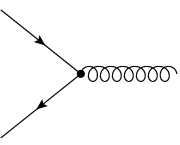
\includegraphics[width=0.35\textwidth]{images/Theory/QCDvertex.png}
    \caption{A Fundamental QCD vertex}
    \label{fig:QCDvertex}
\end{center}
\end{figure}


Equation~\ref{eqn:QCDL} gives the QCD lagrangian where $G_{\mu \nu }^{a}=\partial _{\mu }{\mathcal {A}}_{\nu }^{a}-\partial _{\nu }{\mathcal {A}}_{\mu }^{a}+gf^{abc}{\mathcal {A}}_{\mu }^{b}{\mathcal {A}}_{\nu }^{c}$ is the gluon field strength tensor and $f^{abc}$ are the structure constants of SU(3).
\begin{equation}
    \label{eqn:QCDL}
{\mathcal {L}}_{\mathrm {QCD} }={\bar {\psi }}_{i}\left(i(\gamma ^{\mu }D_{\mu })_{ij}-m\,\delta _{ij}\right)\psi _{j}-{\frac {1}{4}}G_{\mu \nu }^{a}G_{a}^{\mu \nu }
\end{equation}

\textbf{Asymptotic freedom and colour confinement}\\
Quark-antiquark loops lead to screening of the quark colour charge, however gluon loops contribute the opposite by `anti-screening'. The global effect is captured in Eq.~\ref{eqn:alphaSQCD} where it can be seen that in any theory with $11n>2f$, the coupling constant, $\alpha_{S}\left( |q^{2}| \right)$, will decrease with increasing energy, q$^{2}$. This is known as \emph{asymptotic freedom} and so the quarks inside hadrons effectively act like free particles.

\begin{equation}
\label{eqn:alphaSQCD}
\alpha_{S}\left( |q^{2}| \right) = \frac{\alpha_{S}\left( \mu^{2} \right)} {1 + \left[ \alpha_{S}\left( \mu^{2} \right)/12\pi \right]\left( 11n -2f \right) \ln \left(|q^{2}|/\mu^{2}\right)}
\end{equation}

At larger distances the strong force increases, hence energy which has gone into separating two quarks reaches a critical point where it is transferred into producing more quarks which accompany the separated quarks to form hadrons. This is the principle of \emph{confinement} and it ensures that colour doubles or octets are never found in nature, only colour singlet states such as mesons and baryons. The showering of separated quarks into hadrons is called \emph{hadronisation}.


\section{Proton-proton collisions}
At a lepton collider, one can assume that the initial particles involved in a collision are fundamental particles which means precise details of the initial state are known. However at the Large Hadron Collider (LHC) the particles involved in the collisions are protons, which are much more complex composite particles consisting of three valence quarks (two up quarks and one down quark) and gluons which exchange the strong force, as well as `sea quarks' which are quark-anti-quark pairs which come into and out existence rapidly and continuously within the proton.

Figure~\ref{fig:protonPDF} shows the parton distribution functions for the proton. These are interpreted as the probability for a quark to be carrying a fraction, $x$, of the proton's momentum in the longitudinal direction.

\begin{figure}[ht!]
\begin{center}
    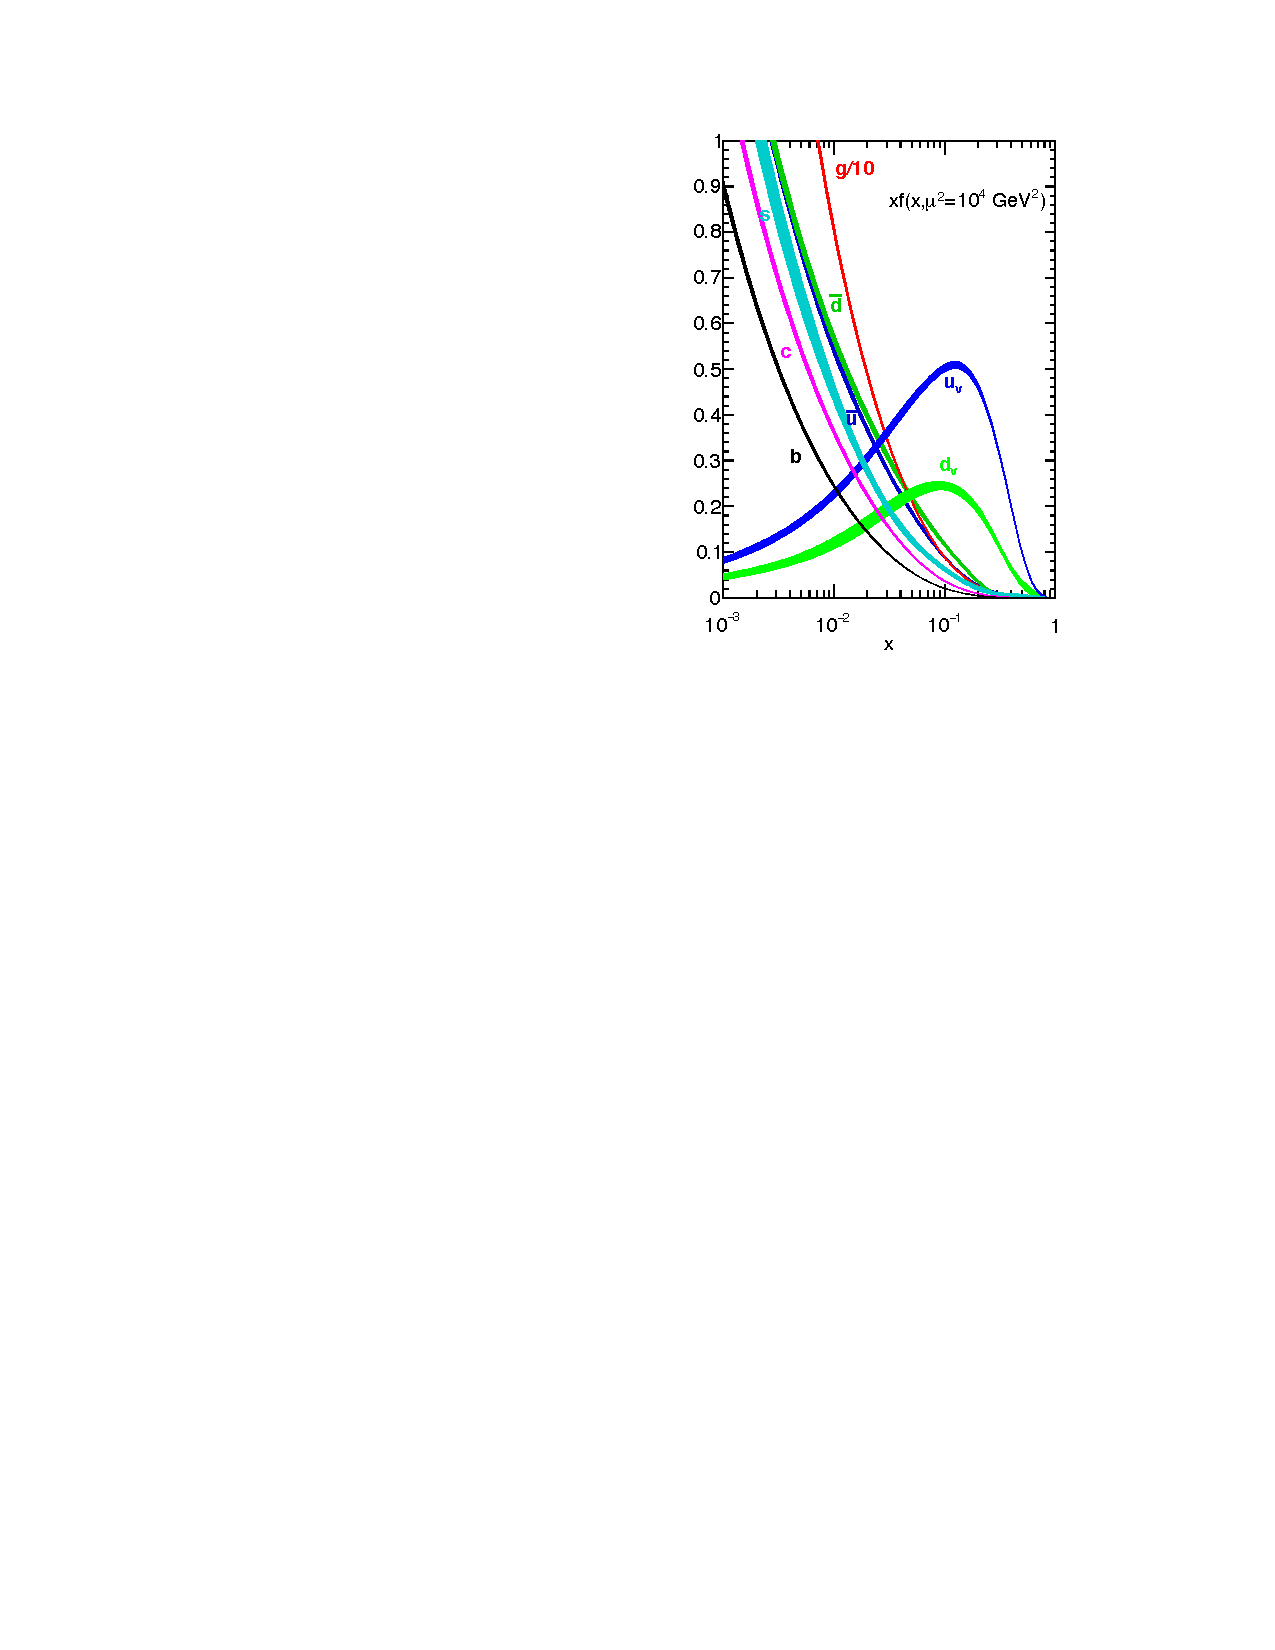
\includegraphics[width=0.49\textwidth]{images/Theory/pdf3.pdf}
    \caption{Proton parton distribution functions f(x) $(f = u_{v},~ d_{v},~ \overline{u},~ \overline{d},~ s\approx\overline{s},~ c\approx\overline{c},~ b\approx\overline{b},~ g$ ) for a given momentum fraction, x. Obtained from NNLO NNPDF3.0~\cite{Ball2015}}
    \label{fig:protonPDF}
\end{center}
\end{figure}

The protons may a) not interact at all and continue to be accelerated around the LHC, b) interact via a soft scatter where the products mostly travel along the direction of the beam, c) participate in a hard interaction where two partons within the protons have a high energy collision with products which travel transverse to the beam. In the latter case, the remaining partons which have not participated in the hard interaction hadronise and form what is known as the \emph{underlying event} (UE)


\section{Four top quark production}

The production of four top quarks occurs predominantly via gluon fusion, as seen at leading order in Fig.~\ref{fig:ttttAtLO}~(left), with a $10\%$ contribution from quark-anti-quark annihilation. The production mechanism occurs via QCD whereas the decay of top quarks via W bosons is a weak interaction. 

\begin{figure}[ht!]
\begin{center}
    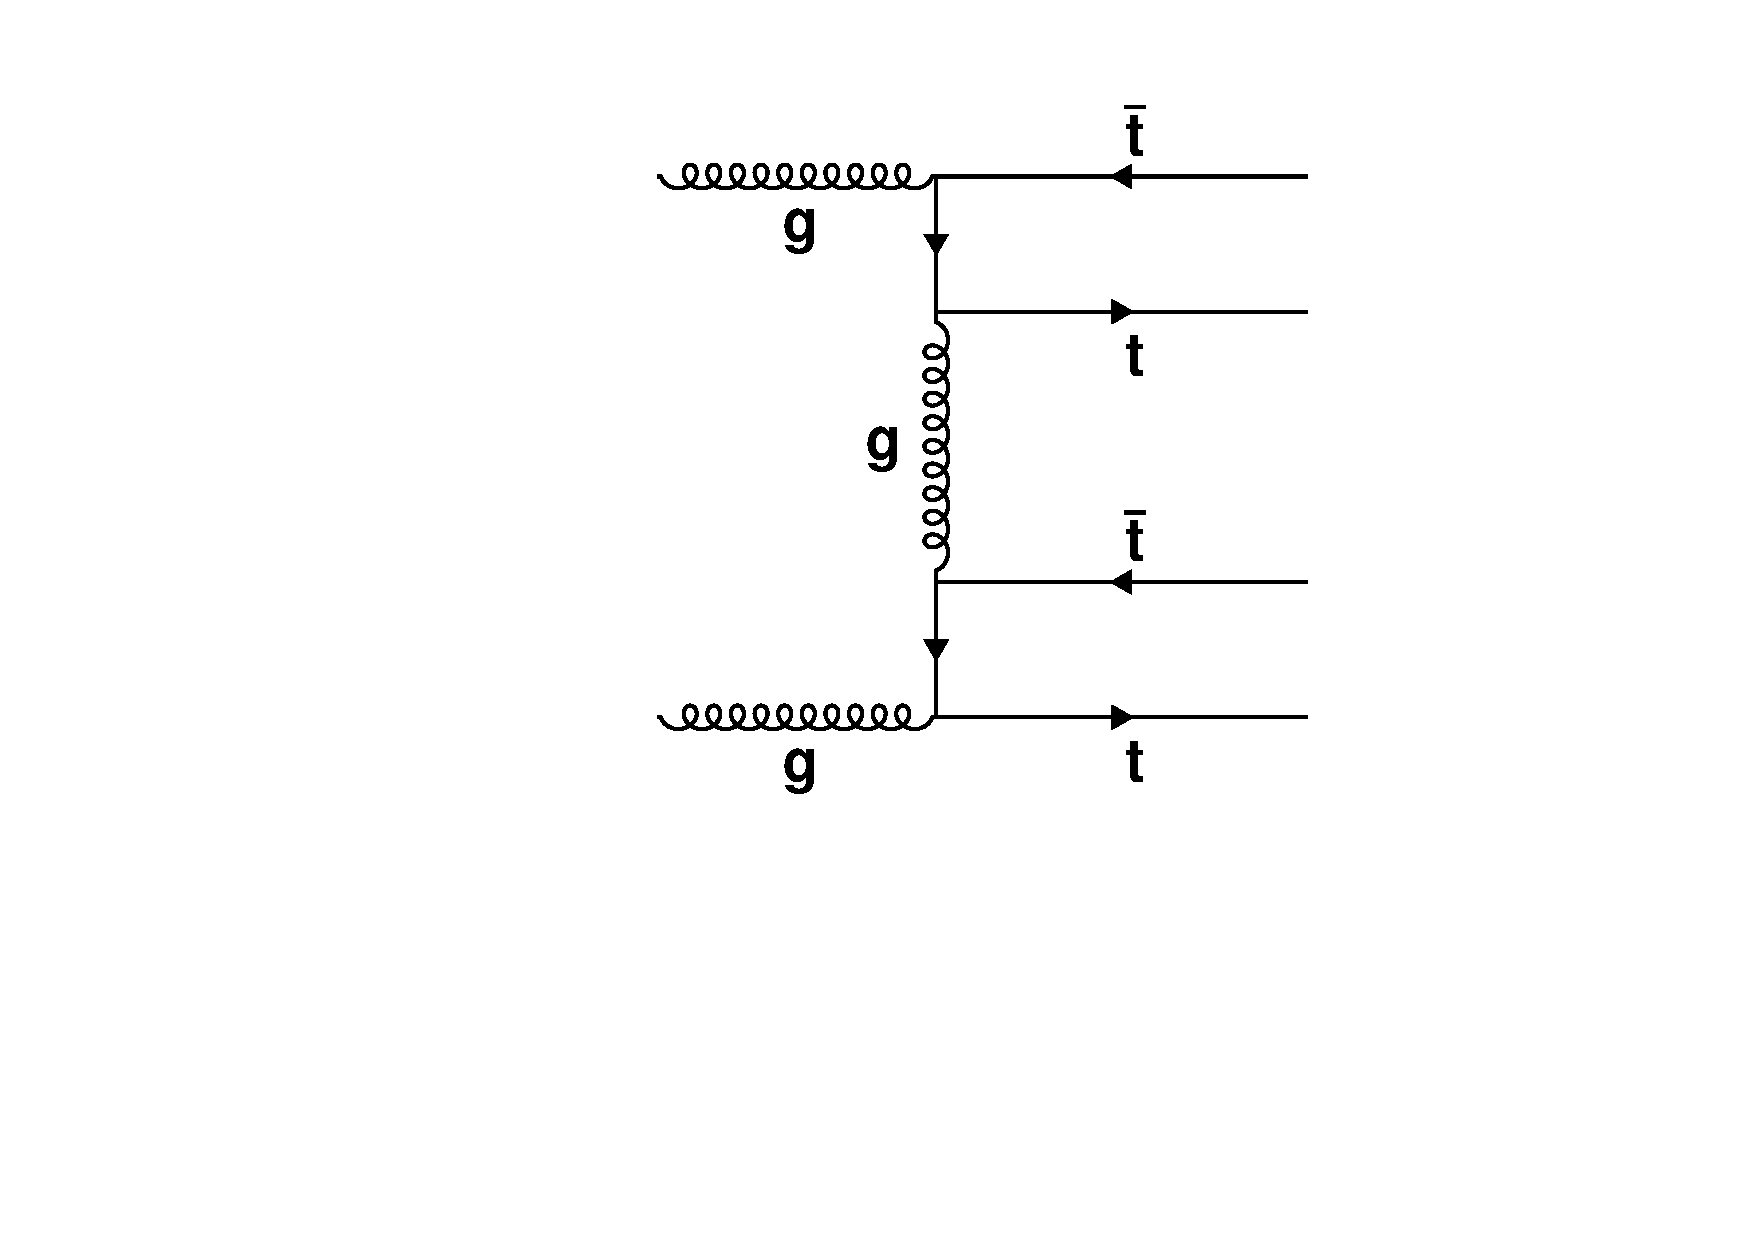
\includegraphics[width=0.49\textwidth]{images/Theory/tttt_t_LO.pdf}
    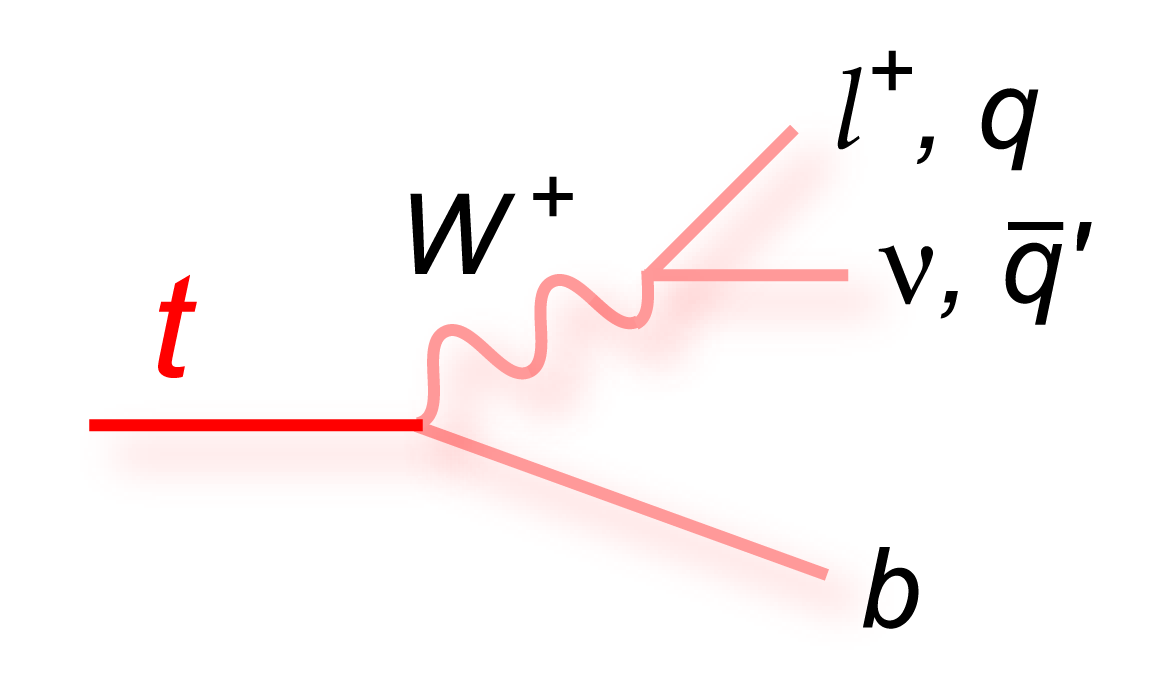
\includegraphics[width=0.49\textwidth]{images/Theory/topdecay.png}
    \caption{Dominant production mechanism for four top quarks in the standard model (left) an top quark decay to a W boson and b-quark with subsequent decay of the W boson either leptonically or hadronically (right).}
    \label{fig:ttttAtLO}
\end{center}
\end{figure}

Final states are determined by the decay of the W boson which can occur either leptonically or hadronically as seen in Fig.~\ref{fig:ttttAtLO}~(right). It can be seen from Fig.~\ref{fig:BRtttt} that the single lepton final state has the largest branching ratio which makes it a favourable place to look to study the largest number of events produced in the CMS detector. This is the final state considered most in this thesis. The dilepton final state also has a large branching ratio and has particularly low backgrounds when same-sign lepton final states are considered. The combination of studies on the dilepton final state will be discussed in the Chapter~\ref{c:Run2}.

\begin{figure}[ht!]
\begin{center}
    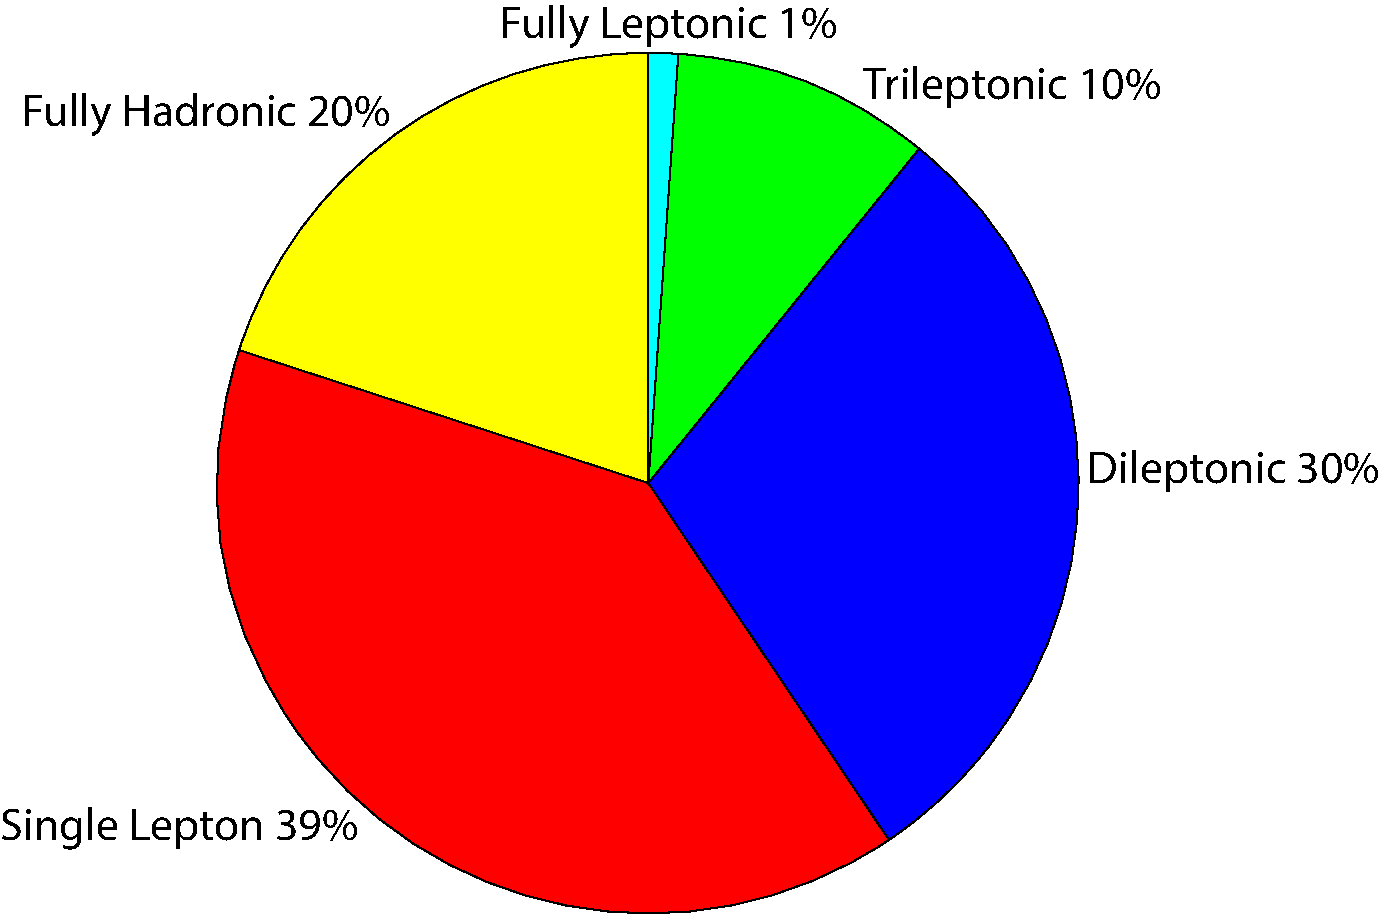
\includegraphics[width=0.4\textwidth]{images/Theory/FourTopBR.pdf}
    \caption{Branching ratios for final states as defined by leptonic decays.}
    \label{fig:BRtttt}
\end{center}
\end{figure}

Figure~\ref{fig:tttt100tev} shows the cross section for \tttt production versus centre of mass energy, $\sqrt{s}$, in the proton-proton collision. It can be seen that the cross section rises with energy and indeed it increases faster than the main background of \ttbar production which means that the signal to background ratio increases with $\sqrt{s}$. Table~\ref{tab:xsec} shows the cross sections for \tttt production and \ttbar production where it can be seen that the \tttt cross section increases by a factor of $\approx~7$ from $\sqrt{s} = 8$~TeV to $\sqrt{s} = 13$~TeV whereas the \ttbar production increase by a factor of $\approx~3.5$.

\begin{figure}[ht!]
\begin{center}
    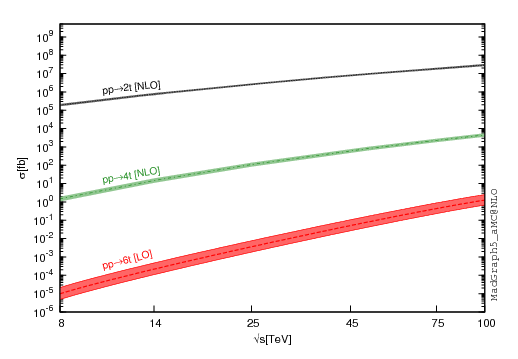
\includegraphics[width=0.95\textwidth]{images/Theory/100TeV.png}
    \caption{The \ttbar (2t), four top quark (4t) and six top quark (6t) production cross sections at a range of $\sqrt{s}$ energies}
    \label{fig:tttt100tev}
\end{center}
\end{figure}

\begin{table}[]
\centering
% \caption{My caption}
\label{tab:xsec}
\begin{tabular}{|l|l|l|}
\hline
Cross section & 8~TeV (\pb) & 13~TeV (\pb) \\ \hline
\tttt         & 0.0013           & 0.0092            \\ \hline
\ttbar        & 245              & 831               \\ \hline
\end{tabular}
\end{table}

\subsection{\ttbar background}

The main background to \tttt production is \ttbar. In the case of the single lepton channel, semi-leptonic \ttbar, where one of the top quarks decays hadronically and the other top quark decays leptonically, is the main final state which contributes to the background. Figure~\ref{fig:ttbarback} shows semi-leptonic \ttbar production with initial and final state radiation. Initial state radiation (ISR) refers to any particle which is radiated off of an incoming particle to the collision whereas final state radiation (FSR) refers to a particle radiated off the final state outgoing products of a collision.

\begin{figure}[ht!]
\begin{center}
    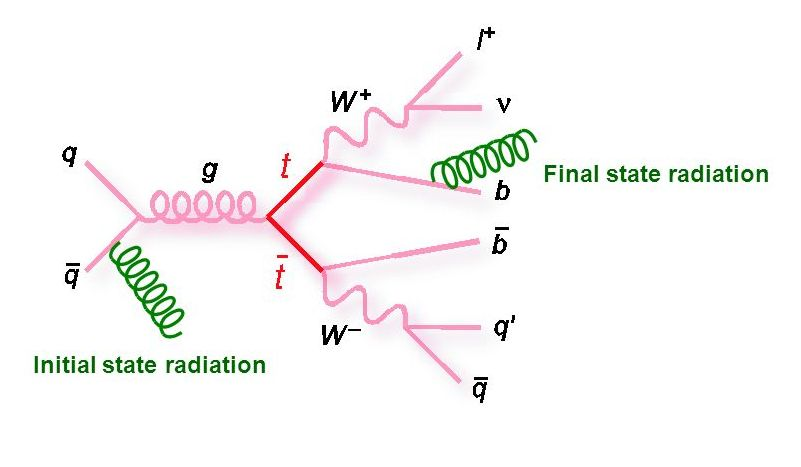
\includegraphics[width=0.95\textwidth]{images/Theory/ttbarISRFSR.jpg}
    \caption{Semi-leptonic \ttbar production with demonstration of extra jets arising from initial and final state radiation}
    \label{fig:ttbarback}
\end{center}
\end{figure}

The semi-leptonic \ttbar process can produce final states which look very much like a \tttt final state in the detector. There are two top quarks which will produce hard jets including two b-quark jets and one lepton. There are also the additional jets from ISR and FSR which increase the jet multiplicity in the event. As in all collisions, final state jets may arise that do not exceed the \pt threshold of the trigger, which is described in Section~\ref{det:trigger}. Jets may also fall outside of the acceptance of the detector or jets may merge together both of which can lower the \tttt multiplity to look more like \ttbar. 
The spectrum of `additional jets' which are not associated with coming from the decay of a top quark are shown in Fig.~\ref{fig:ttbarAdd} for a CMS analysis at $\sqrt{s}=13$~TeV. Event which lie in the tail of the additional jets distribution are more likely to fall within the requirements for a \tttt event. However, in general, jets which come from ISR or FSR tend to be \emph{softer}, ie. lower in \pt.

\begin{figure}[ht!]
\begin{center}
    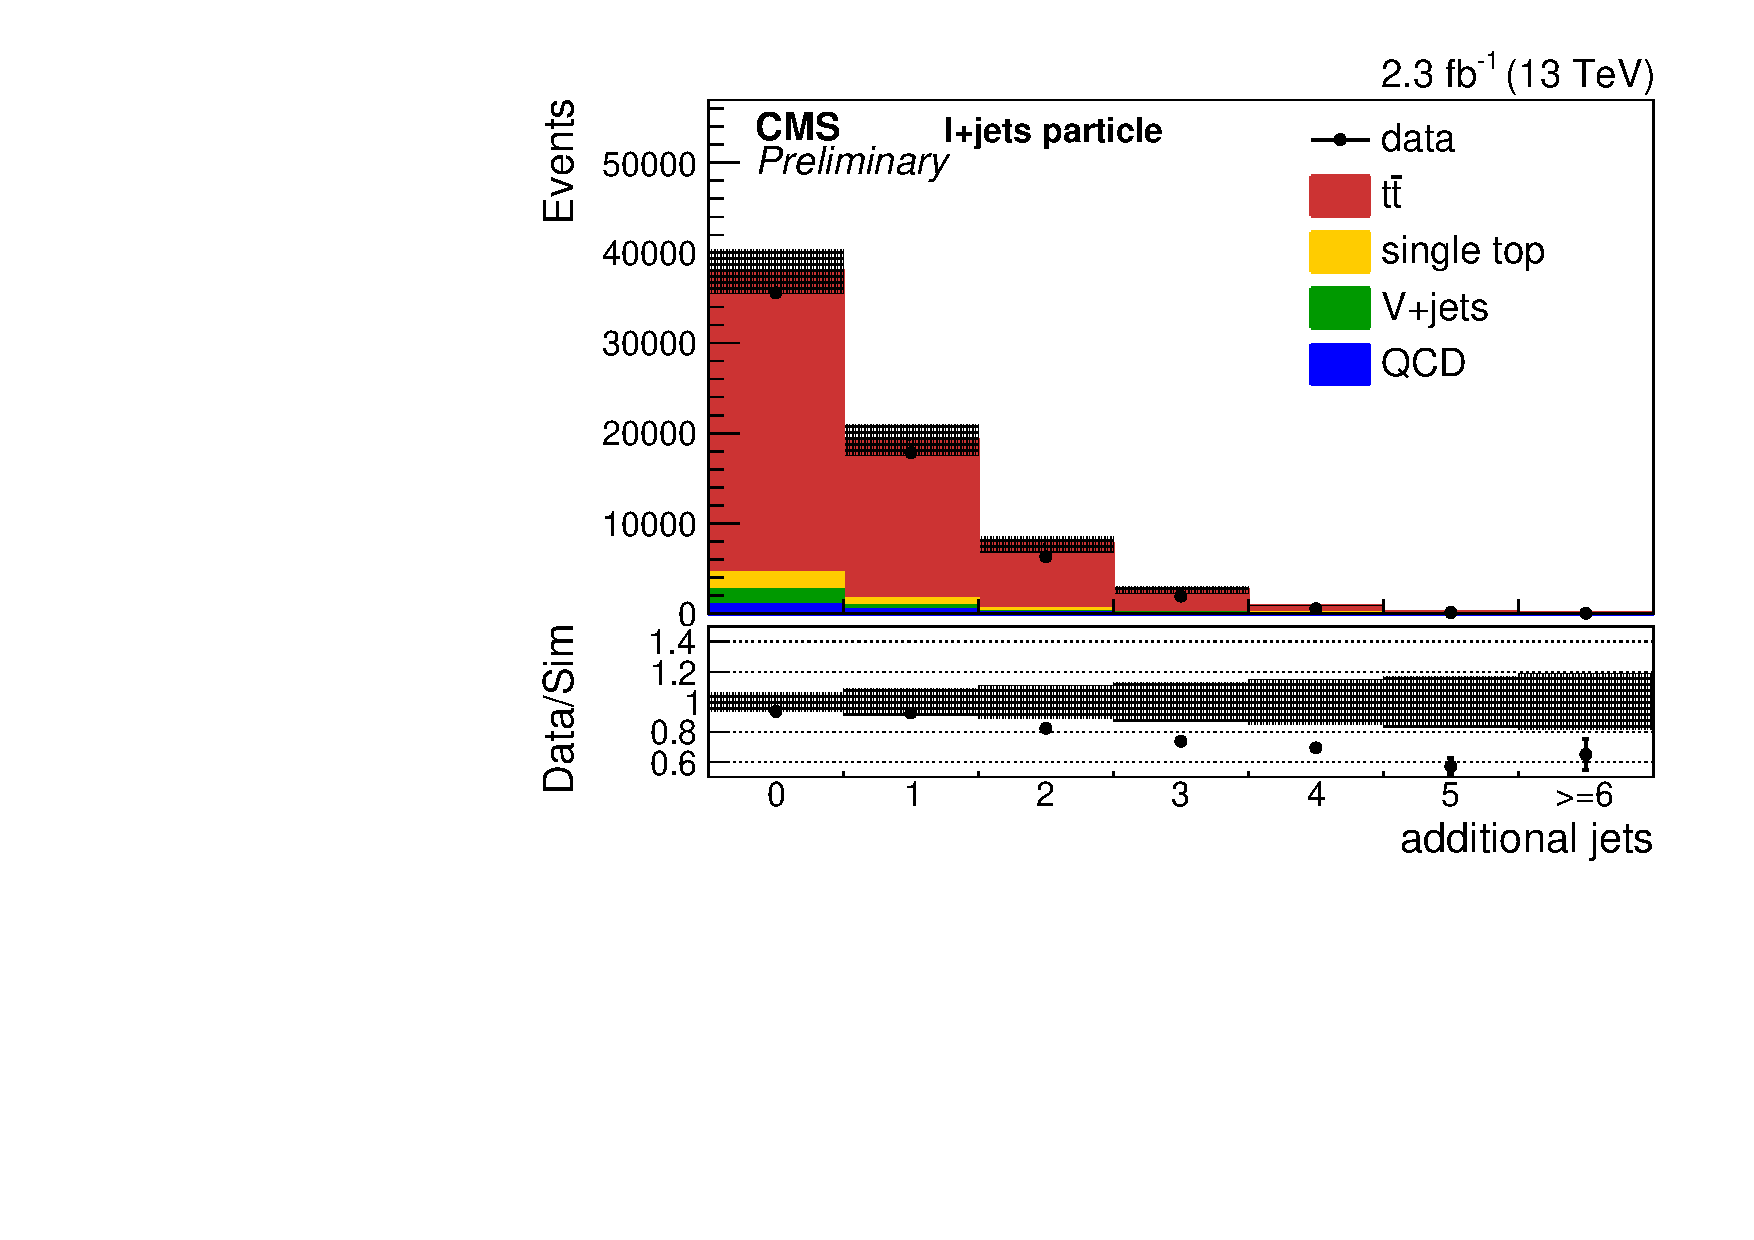
\includegraphics[width=0.85\textwidth]{images/Theory/ttbarAdd.pdf}
    \caption{Jet multiplicity }
    \label{fig:ttbarAdd}
\end{center}
\end{figure}

\subsection{Electroweak backgrounds}

\subsection{Rarer backgrounds}

\section{Shortcomings in the standard model}

\section{BSM models with four top quark signatures}



